% Slide 42: Model Evaluation Introduction
\begin{frame}{ارزیابی مدل‌های طبقه‌بندی}{\lr{Model Evaluation: Generalization Performance}}
  \begin{itemize}
    \setlength{\itemsep}{12pt}
    \item \textbf{پرسش بنیادین در ارزیابی مدل:}
    \begin{itemize}
      \item یک مدل تا چه اندازه در طبقه‌بندی رکوردهای جدید و نادیده (\lr{Unseen Records}) موفق عمل می‌کند؟ (\textbf{کارایی تعمیم} یا \lr{Generalization Performance}).
    \end{itemize}
    \item \textbf{معیارهای ارزیابی در برابر روش‌های ارزیابی:}
    \begin{itemize}
      \setlength{\itemsep}{4pt}
      \item \textbf{معیارهای ارزیابی:} \lr{(Evaluation Metrics)} چگونه کیفیت عملکرد یک مدل را با اعداد و مقادیر کمی بسنجیم؟ (صحت، دقت، بازخوانی، $F_1$، منحنی ROC).
      \item \textbf{روش‌های ارزیابی:} \lr{(Evaluation Methods)} چگونه نمونه‌های داده را تفکیک کنیم تا تخمینی \textbf{قابل‌اعتماد و بدون سوگیری} از کارایی تعمیم به دست آوریم؟
    \end{itemize}
  \end{itemize}
\end{frame}

% Slide 43: General Approach & Golden Rule
\begin{frame}{رویکرد عمومی تفکیک داده}{قاعده زرین ارزیابی مدل}
  \begin{itemize}
    \setlength{\itemsep}{8pt}
    \item تفکیک رکوردهای برچسب‌دار به دو زیرمجموعه مجزا: \textbf{مجموعه آموزش (\lr{Training Set})} و \textbf{مجموعه آزمون (\lr{Test Set})}.
    \item \textbf{قاعده زرین و حیاتی در علم داده:}
    \begin{itemize}
      \item \textcolor{red}{\textbf{هرگز و تحت هیچ شرایطی، مدلی را روی داده‌های آموزش‌دیده ارزیابی نکنید!}}
      \item ارزیابی روی داده‌های آموزش به دلیل برازش مدل، معیاری کاملاً غیرواقع‌بینانه و بیش‌ازحد خوش‌بینانه از عملکرد روی داده‌های آینده خواهد داد.
      \item باید جداسازی فیزیکی و منطقی کاملی میان داده‌های آموزش و آزمون وجود داشته باشد.
    \end{itemize}
    \item \textbf{روش‌های تفکیک متداول:}
    \begin{itemize}
      \item روش نگه‌داشت (\lr{Holdout Method})
      \item زیرنمونه‌گیری تصادفی (\lr{Random Subsampling})
      \item اعتبارسنجی متقاطع (\lr{Cross-Validation})
    \end{itemize}
  \end{itemize}
\end{frame}

% Slide 44: Learning Curve
\begin{frame}{منحنی یادگیری}{\lr{Learning Curve}}
  \begin{columns}[T]
    \begin{column}{0.54\textwidth}
      \begin{itemize}
        \setlength{\itemsep}{8pt}
        \item منحنی یادگیری تغییرات صحت مدل را با \textbf{افزایش حجم داده‌های آموزشی} نشان می‌دهد.
        \item \textbf{نتایج کلیدی:}
        \begin{itemize}
          \setlength{\itemsep}{3pt}
          \item اگر عملکرد مدل پایین یا ناپایدار است، داده‌های آموزشی بیشتری اضافه کنید.
          \item ترجیح بر این است که داده‌های برچسب‌دار را بیشتر به آموزش اختصاص دهیم تا آزمون.
        \end{itemize}
        \item \textbf{چالش عملی:} برچسب‌گذاری نمونه‌های اضافی نیازمند نیروی انسانی متخصص و هزینه مالی بالاست.
      \end{itemize}
    \end{column}
    \begin{column}{0.44\textwidth}
      \begin{center}
        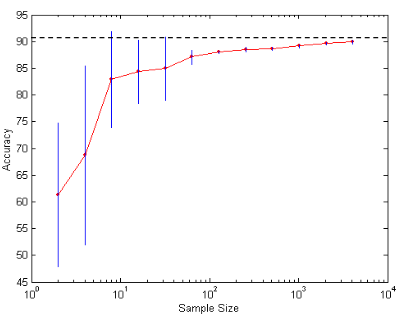
\includegraphics[width=\textwidth,height=4.8cm,keepaspectratio]{images/slide44_learning_curve_clean.png}
      \end{center}
    \end{column}
  \end{columns}
\end{frame}

% Slide 45: Holdout Method
\begin{frame}{روش نگه‌داشت}{\lr{Holdout Method}}
  \begin{itemize}
    \setlength{\itemsep}{4pt}
    \item \textbf{روش نگه‌داشت:} بخش معینی از داده‌های برچسب‌دار را صرفاً برای آزمون ذخیره کرده و از مابقی جهت آموزش استفاده می‌کند:
    \begin{itemize}
      \item زمانی به کار می‌رود که \textbf{حجم زیادی از داده‌های نمونه} در دسترس باشد.
    \end{itemize}
    \item \textbf{نسبت‌های معمول تفکیک:} \lr{2/3} به \lr{1/3} (یا ترجیحاً \lr{80\%} به \lr{20\%}).
  \end{itemize}
  \vspace{0.1cm}
  \begin{center}
    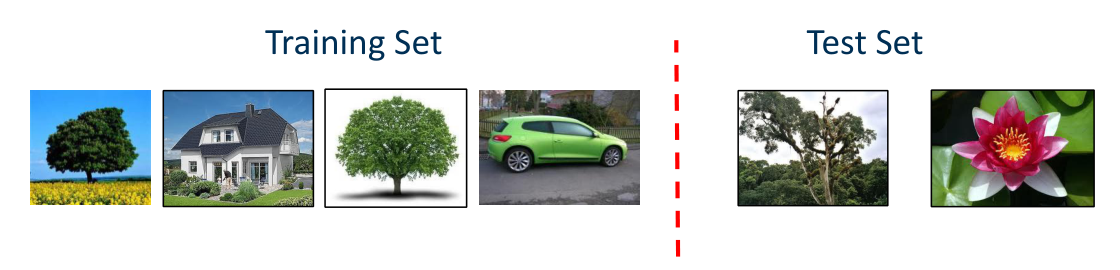
\includegraphics[width=0.80\textwidth,height=2.2cm,keepaspectratio]{images/slide45_holdout_method.png}
  \end{center}
  \vspace{0.05cm}
  \begin{itemize}
    \setlength{\itemsep}{3pt}
    \item در \textbf{مجموعه‌داده‌های نامتعادل}، نمونه‌های تصادفی ممکن است نماینده مناسبی نباشند:
    \begin{itemize}
      \item حضور اندک یا عدم حضور کلاس اقلیت (کلاس مثبت) در آموزش یا آزمون.
    \end{itemize}
  \end{itemize}
\end{frame}

% Slide 46: Stratified Sampling
\begin{frame}{نمونه‌گیری طبقه‌بندی‌شده}{\lr{Stratified Sampling}}
  \begin{itemize}
    \setlength{\itemsep}{5pt}
    \item \textbf{نمونه‌گیری طبقه‌بندی‌شده} (\lr{Stratified Sample}): نمونه‌گیری از هر کلاس به صورت کاملاً مستقل انجام می‌شود تا رکوردهای کلاس اقلیت در تمام نمونه‌ها حضور داشته باشند:
    \begin{itemize}
      \setlength{\itemsep}{3pt}
      \item اطمینان از اینکه هر کلاس با نسبت‌های تقریباً یکسان در هر دو زیرمجموعه حضور دارد.
      \item سایر ویژگی‌ها نیز می‌توانند مبنای طبقه‌بندی قرار گیرند (مانند جنسیت، سن و غیره).
    \end{itemize}
  \end{itemize}
  \vspace{0.1cm}
  \begin{center}
    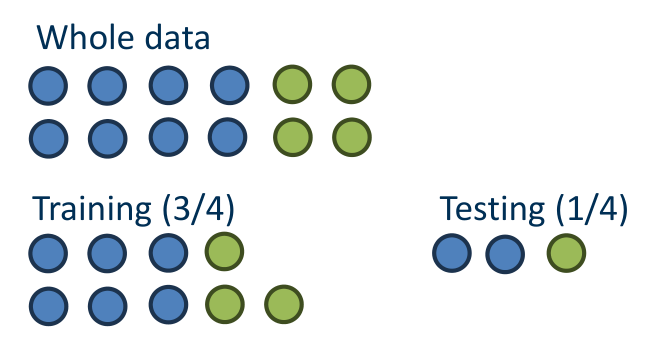
\includegraphics[width=0.85\textwidth,height=2.9cm,keepaspectratio]{images/slide46_stratified_sampling.png}
  \end{center}
\end{frame}

% Slide 47: Random Subsampling
\begin{frame}{زیرنمونه‌گیری تصادفی}{\lr{Random Subsampling}}
  \begin{itemize}
    \setlength{\itemsep}{2pt}
    \item برآورد روش نگه‌داشت را می‌توان با تکرار فرآیند با زیرنمونه‌های مختلف قابل‌اعتمادتر کرد:
    \begin{itemize}
      \item در هر تکرار، درصد معینی به صورت تصادفی برای آموزش انتخاب می‌شود.
      \item میانگین عملکرد تکرارهای مختلف به دست می‌آید.
    \end{itemize}
  \end{itemize}
  \vspace{0.05cm}
  \begin{center}
    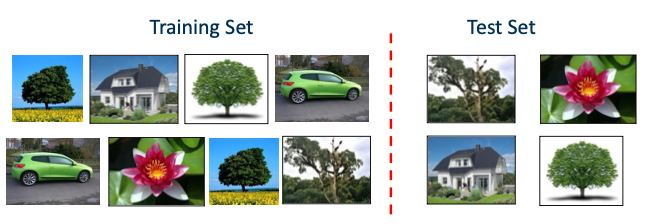
\includegraphics[width=0.78\textwidth,height=2.6cm,keepaspectratio]{images/slide47_random_subsampling_clean.png}
  \end{center}
  \vspace{0.05cm}
  \begin{itemize}
    \setlength{\itemsep}{2pt}
    \item همچنان کاملاً بهینه نیست زیرا مجموعه‌های آزمون ممکن است هم‌پوشانی داشته باشند:
    \begin{itemize}
      \item برخی داده‌های پرت ممکن است همواره در مجموعه‌های آزمون قرار گیرند.
      \item نمونه‌های مهم برای یادگیری ممکن است مکرراً فقط در مجموعه آزمون بیفتند.
    \end{itemize}
  \end{itemize}
\end{frame}

% Slide 48: Leave-One-Out Cross Validation
\begin{frame}{روش تک‌نمونه نگه‌داشته}{\lr{Leave-One-Out (LOO)}}
  \begin{itemize}
    \setlength{\itemsep}{10pt}
    \item حالت حدی اعتبارسنجی: در هر گام، مدل روی $N-1$ نمونه آموزش دیده و روی تنها \textbf{یک نمونه} ارزیابی می‌شود (تکرار $N$ بار برای تمامی رکوردهای داده).
    \item \textbf{مزایا:} دقیق‌ترین برآورد ممکن با کمترین سوگیری، و حداکثر بهره‌برداری از داده‌ها برای آموزش.
    \item \textbf{چالش محاسباتی عظیم:}
    \begin{itemize}
      \item در مجموعه داده با یک میلیون نمونه، اگر آموزش هر مدل تنها ۱ دقیقه زمان ببرد، اجرای روش \lr{LOO} نزدیک به ۲ سال طول خواهد کشید!
    \end{itemize}
  \end{itemize}
\end{frame}

% Slide 49: Cross-Validation
\begin{frame}{اعتبارسنجی متقاطع \lr{$k$-Fold}}{\lr{k-Fold Cross-Validation}}
  \begin{itemize}
    \setlength{\itemsep}{5pt}
    \item تعادلی بهینه میان دقت تخمین روش \lr{LOO} و زمان اجرای منطقی.
    \item \textbf{مرحله اول:} داده‌ها به $k$ زیرمجموعه مساوی و مجزا (\lr{Folds}) با نمونه‌گیری طبقه‌بندی‌شده افراز می‌شوند.
    \item \textbf{مرحله دوم:} در $k$ تکرار، هر زیرمجموعه یک بار برای آزمون و $k-1$ زیرمجموعه باقیمانده برای آموزش به کار می‌روند؛ نهایتاً میانگین خطاها محاسبه می‌شود.
  \end{itemize}
  \vspace{0.1cm}
  \begin{center}
    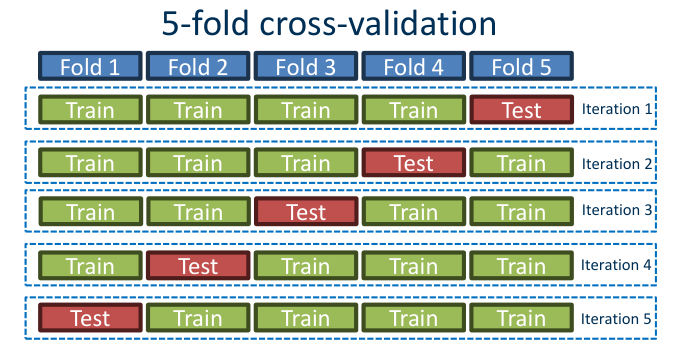
\includegraphics[width=0.88\textwidth,height=3.6cm,keepaspectratio]{images/slide49_cross_validation.png}
  \end{center}
\end{frame}

% Slide 50: Choosing k & Scikit-learn
\begin{frame}{انتخاب مقدار \lr{$k$} و پیاده‌سازی در پایتون}{\lr{Cross-Validation in Scikit-Learn}}
  \begin{itemize}
    \setlength{\itemsep}{4pt}
    \item \textbf{انتخاب مقدار پیش‌فرض} ($k = 10$): تجربیات گسترده نشان داده $k=10$ تعادل بسیار عالی از نظر واریانس و سوگیری برآورد خطا فراهم می‌کند.
    \item در مدل‌های بسیار بزرگ و سنگین امروزی، مقادیر کمتر نظیر $k=5$ (مقدار پیش‌فرض \lr{scikit-learn}) ترجیح داده می‌شود.
    \item \textbf{پیاده‌سازی نمونه‌گیری طبقه‌بندی‌شده (\lr{Stratified}) در پایتون:}
  \end{itemize}
  \vspace{0.1cm}
  \begin{latin}
    \begin{minipage}{0.96\textwidth}
      \fcolorbox{codeborder}{codebg}{%
        \begin{minipage}{0.97\textwidth}
          \ttfamily\small
          \textbf{from} sklearn.model\_selection \textbf{import} StratifiedKFold, cross\_val\_score\\[4pt]
          \textcolor{mannheimteal}{\# Configure stratified 10-fold split with shuffling}\\
          cross\_val = StratifiedKFold(n\_splits=10, shuffle=\textbf{True}, random\_state=42)\\[4pt]
          \textcolor{mannheimteal}{\# Compute cross-validation accuracy across all 10 folds}\\
          accuracy = cross\_val\_score(estimator, data, target, cv=cross\_val, scoring=\textcolor{teal}{'accuracy'})
        \end{minipage}%
      }
    \end{minipage}
  \end{latin}
\end{frame}
